%auto-ignore
\documentclass{standalone}

\usepackage{graphicx}
\usepackage{tikz}

\begin{document}
\begin{tikzpicture}
\node[inner sep=0pt,label=left:{$i + 1$}]
(fapl3) at (0,0)
	{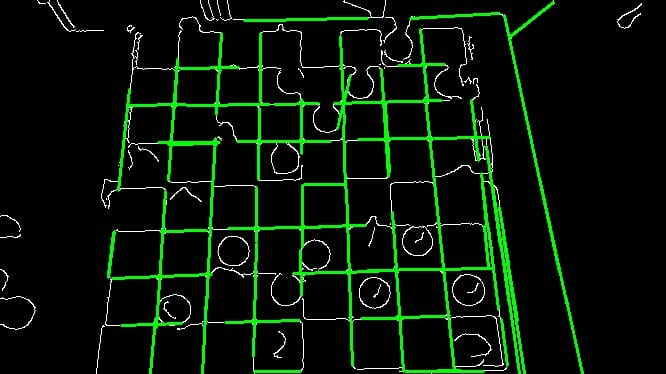
\includegraphics[width=.25\textwidth]{figure4_i3.jpg}};
\node[inner sep=0pt,label=left:{$i$}]
(fapl2) at (0,3)
	{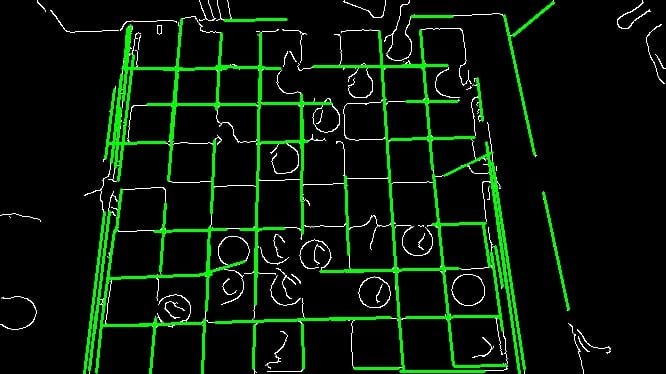
\includegraphics[width=.25\textwidth]{figure4_i2.jpg}};
\node[inner sep=0pt,label=left:{$i - 1$}]
(fapl1) at (0,6)
	{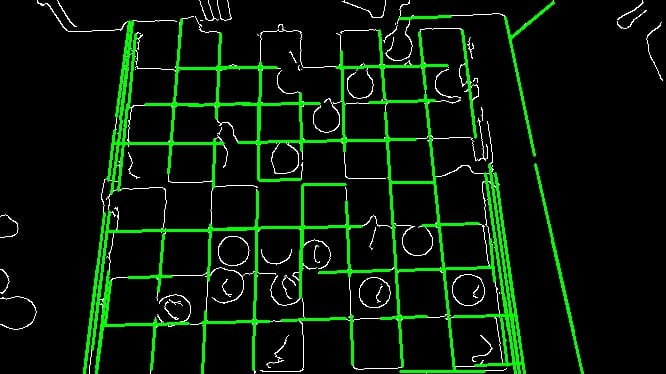
\includegraphics[width=.25\textwidth]{figure4_i1.jpg}};
\node[inner sep=0pt,label={[yshift=0.50cm]\textbf{all}}]
(fapl_all) at (8,3)
	{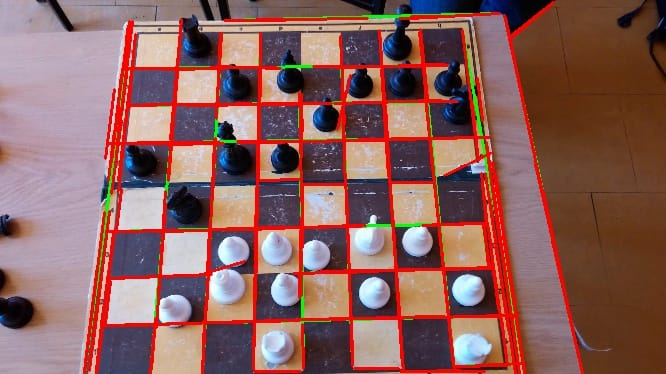
\includegraphics[width=.50\textwidth]{figure4_a.jpg}};
\node[inner sep=0pt,label={[yshift=0.50cm]\textbf{heated}}]
(fapl_lines) at (17,3)
	{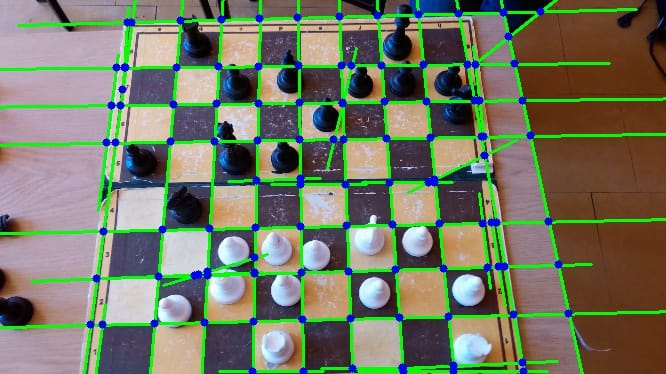
\includegraphics[width=.50\textwidth]{figure4_b.jpg}};
\draw[->,thick,shorten >=6pt,shorten <=6pt] (fapl1) -- (fapl_all)
	node[midway,fill=white,align=center] {overexposed};
\draw[->,thick,shorten >=6pt,shorten <=6pt] (fapl2) -- (fapl_all)
	node[midway,fill=white,align=center] {blurred};
\draw[->,thick,shorten >=6pt,shorten <=6pt] (fapl3) -- (fapl_all)
	node[midway,fill=white,align=center] {tinted};
\draw[->,thick,shorten >=6pt,shorten <=6pt] (fapl_all) -- (fapl_lines)
	node[midway,fill=white,align=center] {thermal\\analysis};
\end{tikzpicture}
\end{document}
